\documentclass{beamer}
\usepackage{beamerthemesplit}
\usepackage{graphicx,url}
\usepackage[brazil]{babel}
\usepackage[utf8]{inputenc}

\mode<presentation>
{
  \usetheme{Ilmenau}
  \setbeamercovered{transparent}
}

\newcommand{\eng}[1]{\textit{#1}}
\newcommand{\obra}{\textit{Em torno da romã}}

\title{\obra{}: aplicações de operações de contorno na composição}
\author{Marcos da Silva Sampaio}
\date{28 de novembro de 2008}

\logo{\includegraphics[scale=.15]{logo-genos}}

\begin{document}

\frame{\titlepage}

\frame{
  \frametitle{Esta apresentação}
  \tableofcontents
}

\section{Introdução}

\frame{
  \frametitle{O que são contornos?}
  \begin{figure}
    \includegraphics[scale=.6]{roma-pura}
    \hspace{1em}
    \includegraphics[scale=.6]{contorno-com-roma}
  \end{figure}
}

\frame{
  \frametitle{Contornos em Música}
  \begin{figure}
    \centering
    \includegraphics{5a-sinfonia}
  \end{figure}

  \begin{figure}
    \centering
    \includegraphics[scale=1.4]{c-3120}
  \end{figure}
}

\frame{
  \frametitle{Semelhança e coerência}
  \begin{figure}
    \centering
    \includegraphics{ly-2031}
    \hspace{1em}
    \includegraphics[scale=1.4]{c-2031}
  \end{figure}
}

\frame{
  \frametitle{Objetivos e justificativa}
  \begin{itemize}
  \item Justificativa
    \begin{itemize}
    \item Coerência
    \item Manipulação por operações
    \item Estudos escassos
    \end{itemize}
  \item Objetivos
    \begin{itemize}
    \item Composição baseada em operações de contornos
    \item Software para processar contornos
    \item Mapeamento de contornos
    \end{itemize}
  \end{itemize}
}

\section{Contornos}

\frame{
  \frametitle{Definições}
  \begin{figure}
    \centering
    \includegraphics{5a-sinfonia}
  \end{figure}
  \begin{itemize}
  \item Movimento asc./desc. entre elementos adjacentes
    \cite{piston59:harmony,toch77:shaping,edworthy85:musical,dewitt.ea86:recognition}

    (- + -)
  \item Conjunto ordenado numerado ascendentemente \cite{morris93:directions}

    (3 1 2 0)
  \end{itemize}
}

\frame{
  \frametitle{Comparação entre definições}
  Vantagens da definição de Morris:
  \begin{enumerate}
  \item Elementos não adjacentes
  \item Expansível para outros elementos musicais
  \end{enumerate}

  \begin{figure}
    \centering
    \includegraphics[scale=.9]{chord-densities-in-time}
    \hspace{1em}
    \includegraphics[scale=.9]{dynamics-in-time}
    \hspace{1em}
    \includegraphics[scale=1]{c-1023}
  \end{figure}
}

\frame{
  \frametitle{Contornos como determinante composicional}
\begin{figure}
  \centering
    \includegraphics[scale=.7]{webern-tema-analisado}

    \includegraphics[scale=.7]{webern-concatenacao-1}

    \includegraphics[scale=.7]{webern-concatenacao-2}
\end{figure}

}

\frame{
  \frametitle{Representações de contornos}
  \begin{itemize}
  \item Representação simbólica
    \begin{itemize}
    \item Contorno: Z(2 0 3 1)
    \item Elementos: Z$_0=2$, Z$_1=0$, Z$_2=3$ e Z$_3=1$
    \end{itemize}
  \item Representação gráfica
    \begin{figure}
      \centering
      \includegraphics[scale=1.5]{c-2031}
    \end{figure}
  \end{itemize}
}

\frame{
  \frametitle{Representação de operações}
  \begin{itemize}
  \item Retrógrado de X(1 2 3): $retr(X(1\;2\;3))=Y(3\;2\;1)$
  \item Transposição de X(1 2 3) com fator 2: $transp(X(1\;2\;3)\;2)=W(3\;4\;5)$
  \item Concatenação de operações: $transp(retr(inv(rot(X(1\;2\;3))\;2))\;3)$
  \end{itemize}
}

\frame {
  \frametitle{Espaço de contorno}
  \begin{figure}
    \centering
    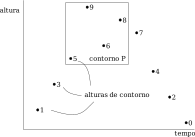
\includegraphics[scale=1.5]{cspace-5968}
  \end{figure}
}

\frame {
  \frametitle{Exemplos de espaço de contorno}
  \begin{figure}
    \centering
    \includegraphics{cspace-564}
    \includegraphics{cspace-7420}
  \end{figure}
}

\frame{
  \frametitle{Operações implementadas}

  Ver direto no Goiaba
}

\section{Goiaba}

\frame{
  \frametitle{}
}

\section{Composição}

\frame{
  \frametitle{}
}

\section{Conclusões}

\frame{
  \frametitle{}
}

\frame[allowframebreaks]{
  \frametitle{Referências}
  \bibliographystyle{alpha}
  \bibliography{melodic-contour,music-perception,composition,music-harmony-and-theory,programs,music-analysis,audio,genos,computer-science}
}

\end{document}
